\documentclass[a4paper,10pt]{ltjsarticle}

% 各種字体
% see http://www.yamamo10.jp/yamamoto/comp/latex/make_doc/formula/amsmath_symbol/index.php
\usepackage{amsmath,amssymb,amsfonts}

% 画像挿入
\usepackage{graphicx}
% 表のボーダー
\usepackage{booktabs}
% ハイパーリンク, URL 挿入
\usepackage[hyphens]{url}
\usepackage{hyperref}
% 色付き文字
\usepackage{xcolor}

% 改ページできるフレーム
\usepackage{framed}

% 単位
% see http://www.yamamo10.jp/yamamoto/comp/latex/make_doc/unit/index.php
\usepackage{siunitx}

%-----------%
% スニペット %
%-----------%

% see https://mirrors.ctan.org/macros/latex/contrib/physics2/physics2.pdf
\usepackage{physics2}
% 自動調整の括弧:\ab() など
\usephysicsmodule{ab}

% 微小量記号:\d など
\usepackage{fixdif}
% 微分記号:\pdv など
\usepackage{derivative}

%-----------%
% コード関連 %
%-----------%

% 疑似コード
% see https://tug.ctan.org/macros/latex/contrib/algorithmicx/algorithmicx.pdf
% see https://qiita.com/tomoyk/items/6016123b5c9034bb0087
\usepackage{algorithm}
\usepackage{algpseudocode}

% コードブロック
% see https://cloudlatex.io/latex-notation#%E3%82%BD%E3%83%BC%E3%82%B9%E3%82%B3%E3%83%BC%E3%83%89
\usepackage{listings}
% \usepackage{jvlisting}

% Global style setting
% see https://nasa.github.io/nasa-latex-docs/html/examples/listing.html
\lstset{
  language={C}, % 載せるソースコードの言語を指定する
  basicstyle={\small}, % 通常のソースのフォントを設定
  identifierstyle={\small},% 変数名などのフォントを設定
  commentstyle={\small\itshape\color[rgb]{0,0.5,0}}, % コメントのフォントを設定
  keywordstyle={\small\bfseries\color[rgb]{0,0,1}}, % 予約語のフォントを設定
  ndkeywordstyle={\small}, % keywordstyle以外に定義されている予約語のフォントを設定
  stringstyle={\small\ttfamily\color[rgb]{1,0,1}}, % 文字列のフォントを設定
  frame={tb}, % 実線で描く枠の位置指定
  breaklines=true, % 自動改行の有無
  columns=[l]{fullflexible},% 文字間の余白
  numbers=left, % 行番号の位置
  numberstyle={\scriptsize}, % 行番号のフォント
  stepnumber=1, % 行番号の刻み幅
  lineskip=-0.5ex, % 行間
}

% インラインコードブロック (\lstinline)
% see https://tex.stackexchange.com/questions/357227/adding-background-color-to-verb-or-lstinline-command-without-colorbox
\usepackage{xpatch}
\usepackage{realboxes}
\definecolor{mygray}{rgb}{0.95,0.95,0.95}
\makeatletter
\xpretocmd\lstinline{\Colorbox{mygray}\bgroup\appto\lst@DeInit{\egroup}}{}{}
\makeatother

%---------%
% 参考文献 %
%---------%

% see https://tex.stackexchange.com/questions/655812/how-to-include-a-url-in-a-customized-way-with-unsrt
\usepackage[numbers, sort]{natbib}
\bibliographystyle{unsrtnat}

%---------------%
% 適宜切り替える %
%---------------%

% 、。と ,. の切り替え (LuaLaTeX 専用)
\usepackage{newunicodechar}
\newunicodechar{、}{,}
\newunicodechar{。}{.}

% ページ数を消す
% \pagestyle{empty}

%---------%
% 文章情報 %
%---------%

\title{サンプル}
%textlint-disable
\author{てすと}
%textlint-enable

\begin{document}

\maketitle
\begin{abstract}
  概要のてすと。
\end{abstract}
\tableofcontents

\section{サンプル}

% see https://tex.stackexchange.com/questions/392168/why-does-chktex-lint-command-terminated-with-space
\LaTeX{} で PDF が作成できます。
textlint で文法がチェックできます。
「本日はは晴天です。」のように助詞が連続すると warning が出ます。
「本日は晴天である。」のように語尾の違いでも warning が出ます。
proofdict を使うと「javascript」のような表記ゆれも確認できます。

itemize 環境などでは ja-technical-writing の
文章区切りがおかしくなるので、
コメントに textlint-disable を記載して無効化しておきます。
% textlint-disable
\begin{itemize}
  \item リンゴは赤
  \item バナナは黄色
  \item ブドウは紫
\end{itemize}
% textlint-enable

AdS/CFT~\cite{maldacena1999large}
の概要を図~\ref{fig:adscft}に示します。
\begin{figure}[tbp]
  \begin{center}
    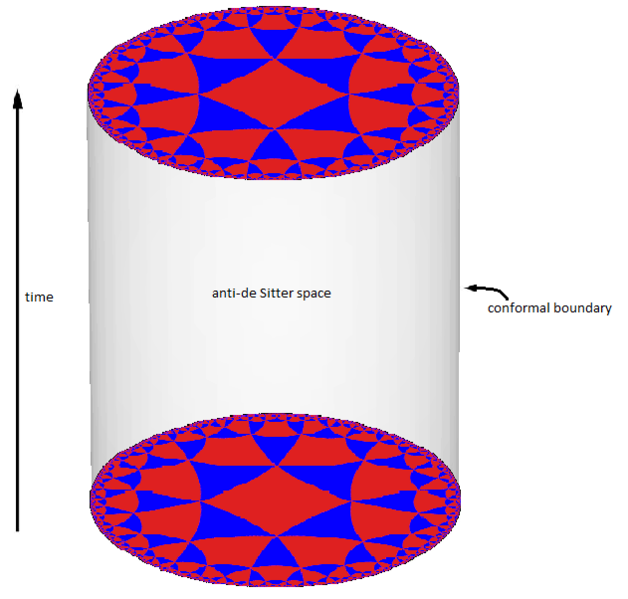
\includegraphics[width=8cm]{img/sample.png}
    \caption{AdS/CFT対応の概念図~\cite{adscftwiki}}
  \end{center}\label{fig:adscft}
\end{figure}
表の作り方を表~\ref{tab:sample}に示します。
\begin{table}[tbp]
  \begin{center}
    \caption{表の例}\label{tab:sample}
    \begin{tabular}{lcc}
      \toprule
      hoge & fuga & piyo \\
      \midrule
      A    & B    & C    \\
      \bottomrule
    \end{tabular}
  \end{center}
\end{table}
アルゴリズム体操はアルゴリズム~\ref{alg:excersise}に示します。
\begin{figure}[tbp]
  \begin{algorithm}[H]
    \caption{アルゴリズム体操}\label{alg:excersise}
    \begin{algorithmic}
      \Function {体操}{}
      \ForAll {こっち, あっち}
      \State {ふたりで まえならえ}
      \EndFor{}
      \EndFunction{}
    \end{algorithmic}
  \end{algorithm}
\end{figure}
インラインのコードブロックは\lstinline|sudo apt update|で書けます。
C++ での Hellow World の実装はソース~\ref{src:hello_world}に示します。
\begin{figure}
  \begin{lstlisting}[caption=Hello World,label={src:hello_world},language=C]
    #include<stdio.h>
    int main(void){
        printf("Hello World!!");
        return 0;
    }
  \end{lstlisting}
\end{figure}

\newpage
\bibliography{reference}

\end{document}